\section{Topologisches Konzept}
Die topologische Überlegung spielt in der Umsetzung eine zentralle Rolle. Die zentrale Aufgabe des Projektes ist es Drohnen zu verwalten, welche sich in einem geografischen Gebiet aufhalten. Dieses Gebiet kann Hindernisse, Gebäude oder Bäume beinhalten, welche möglichst sicher umflogen werden müssen. Da die Drohnen über keine Kollisionserkennung verfügen, ist es umso wichtiger, dass viele Gefahren bereits in der Planung der Mission ausgeschlossen werden kann. Statische Objekte mit unterschiedlicher Höhe können einfach umflogen oder überflogen werden, sofern die Drohne 'weiss' wie diese flugtechnisch zu vermeiden sind. Aus diesen Überlegungen entstand das Zonen Model.
\subsection{Das Zonen Model}

Betrachten wir nun ein einfaches Projekt am Campus der HSR, so könnte dies wie folgt aussehen. \\
\begin{figure}[h]
	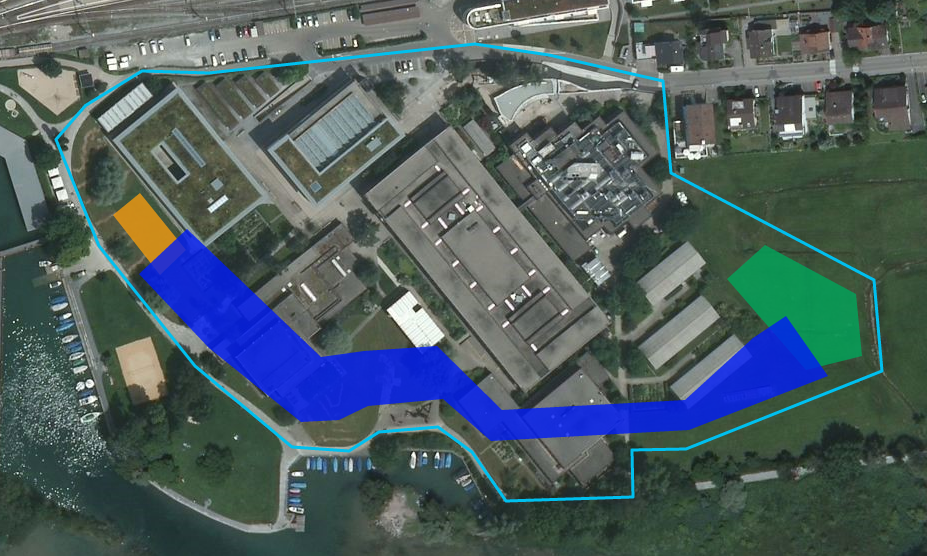
\includegraphics[width=1.0\textwidth]{images/routing/simpleProject_example.png}
	\caption{Einfaches Demo Projekt an der HSR}
	\label{fig:demo-project}
\end{figure}
Jede Farbe kann einer bestimmten Zone zugeteilt werden. Die Zonen können bestimmte Funktionen auf der Drohne auslösen. Zu jeder Zone kann zusätzlich die Höhe hinterlegt werden. Diese gewährleistet die minimale Flughöhe in dem Bereich. Im Falle der DeliveryZone ist die Höhe die Zielhöhe nach dem Start.
\begin{itemize}
	\item{\textbf{OrderZone:} Bereich in welchem Produkte im CustomerApp für dieses Projekt bestellt werden können.  (\textit{hell blauer Rahmen})}
	\item{\textbf{LoadingZone:} Zone die gebraucht wird um die Drohne zu beladen. (\textit{orange})}
	\item{\textbf{DeliveryZone:} Diese Zone definiert das Gebiet über welchem das Produkt abgeworfen werden kann. (\textit{grün})}
	\item{\textbf{FlightZone:} Die Flugzone verbindet die Ladezone mit der Abwurfzone. Weiter garantiert sie, dass die angegebene Flughöhe gewährleistet wird. (\textit{blau})}
\end{itemize}
\subsection{Routing-Algorithmus}


Die Luftraumabbildung in Zonen lässt auf eine Abstraktion in Polygonen schliessen. Polygone sind gut um Bereich zu definieren, aber sie eigenen sich nicht wirklich um eine Route zu B
Die Luftraumaufteilung mit Zonen
Nachdem die Luftraumaufteilung nun mit Zonen gelöst ist, welche durch Polygone abgebildet werden können, muss eine Vereinfachung zu einem Graph gefunden werden, um
Für den Erfolg des Projektes war der Gedanke über die Aufteilung des Luftraums von zentraller Bedeutung. Die Luftraumaufteilung wurde auch relativ schnell mit dem intuitiven Zonen konzept gelöst. Leider sind Zonen, welche quasi durch Polygone abgebildet werden, nicht wirklich gut geeignet um eine Route zu finden. Routing-Algorithmen basieren auf Graphen und nicht auf Polygonen. Schnell waren wir uns bewusst, dass eine erfolgreiche Routenberechnung nicht an einem klassischen Routing Algorithmus vorbei führen würde.
\subsection{Reduktion vom Polygon zum Graph}
Für das Routing sind nur die drei Zonen, LoadingZone, DeliveryZone und FlightZone von entscheidender Bedeutung. Diese Zonen können von der Drohen angeflogen werden, die OrderZone dient nur um die richtigen Produkte im CustommerApp anzuzeigen.